\documentclass[12pt, a4paper]{report}

% ─── Packages ────────────────────────────────────────────────────────────────
\usepackage[utf8]{inputenc}
\usepackage[T1]{fontenc}
\usepackage[english]{babel}
\usepackage{geometry}
\usepackage{graphicx}
\usepackage{xcolor}
\usepackage{amsmath}
\usepackage{amssymb}
\usepackage{booktabs}
\usepackage{longtable}
\usepackage{array}
\usepackage{multirow}
\usepackage{enumitem}
\usepackage{hyperref}
\usepackage{listings}
\usepackage{fancyhdr}
\usepackage{titlesec}
\usepackage{tcolorbox}
\usepackage{tikz}
\usepackage{pgfplots}
\usepackage{float}
\usepackage{caption}
\usepackage{subcaption}
\usepackage{lmodern}
\usepackage{microtype}
\usepackage{setspace}
\usepackage{mdframed}
\usepackage{fontawesome5}

\pgfplotsset{compat=1.18}
\usetikzlibrary{shapes.geometric, arrows.meta, positioning, fit, backgrounds, shadows}

% ─── Page Geometry ────────────────────────────────────────────────────────────
\geometry{
  top=2.5cm, bottom=2.5cm,
  left=2.8cm, right=2.8cm,
  headheight=15pt
}

% ─── Color Palette ────────────────────────────────────────────────────────────
\definecolor{ENSABlue}{HTML}{003F8A}
\definecolor{ENSAGold}{HTML}{C8920A}
\definecolor{ENSALightBlue}{HTML}{E8F0FA}
\definecolor{AccentGreen}{HTML}{1B7A4B}
\definecolor{AccentRed}{HTML}{C0392B}
\definecolor{AccentOrange}{HTML}{D35400}
\definecolor{LightGray}{HTML}{F5F7FA}
\definecolor{MedGray}{HTML}{7F8C8D}
\definecolor{DarkGray}{HTML}{2C3E50}
\definecolor{CodeBg}{HTML}{F0F4F8}
\definecolor{CodeBorder}{HTML}{BDC3C7}

% ─── Hyperref Setup ───────────────────────────────────────────────────────────
\hypersetup{
  colorlinks=true,
  linkcolor=ENSABlue,
  urlcolor=ENSABlue,
  citecolor=ENSABlue,
  pdftitle={Secure BI Architecture -- ENSA Kénitra},
  pdfauthor={ENSA Kénitra},
  bookmarksnumbered=true,
}

% ─── Chapter/Section Styling ──────────────────────────────────────────────────
\titleformat{\chapter}[display]
  {\normalfont\huge\bfseries\color{ENSABlue}}
  {\chaptertitlename\ \thechapter}{18pt}{\Huge}
\titleformat{\section}
  {\normalfont\Large\bfseries\color{ENSABlue}}
  {\thesection}{1em}{}[\color{ENSAGold}\titlerule[1pt]]
\titleformat{\subsection}
  {\normalfont\large\bfseries\color{DarkGray}}
  {\thesubsection}{1em}{}
\titleformat{\subsubsection}
  {\normalfont\normalsize\bfseries\color{MedGray}}
  {\thesubsubsection}{1em}{}

% ─── Header/Footer ────────────────────────────────────────────────────────────
\pagestyle{fancy}
\fancyhf{}
\fancyhead[L]{\small\color{ENSABlue}\textbf{ENSA Kénitra — Secure BI Platform}}
\fancyhead[R]{\small\color{MedGray}\leftmark}
\fancyfoot[C]{\small\thepage}
\fancyfoot[L]{\small\color{MedGray}Academic Year 2024--2025}
\fancyfoot[R]{\small\color{MedGray}Confidential}
\renewcommand{\headrulewidth}{0.8pt}
\renewcommand{\footrulewidth}{0.4pt}

% ─── Code Listing Style ───────────────────────────────────────────────────────
\lstdefinestyle{pythonstyle}{
  backgroundcolor=\color{CodeBg},
  commentstyle=\color{AccentGreen}\itshape,
  keywordstyle=\color{ENSABlue}\bfseries,
  stringstyle=\color{AccentRed},
  basicstyle=\ttfamily\small,
  breakatwhitespace=false,
  breaklines=true,
  keepspaces=true,
  numbers=left,
  numberstyle=\tiny\color{MedGray},
  showspaces=false,
  showstringspaces=false,
  tabsize=4,
  frame=single,
  rulecolor=\color{CodeBorder},
  xleftmargin=15pt,
  xrightmargin=5pt,
  captionpos=b,
}
\lstset{style=pythonstyle}

\lstdefinestyle{sqlstyle}{
  backgroundcolor=\color{CodeBg},
  commentstyle=\color{MedGray}\itshape,
  keywordstyle=\color{AccentOrange}\bfseries,
  stringstyle=\color{AccentGreen},
  basicstyle=\ttfamily\small,
  breaklines=true,
  numbers=left,
  numberstyle=\tiny\color{MedGray},
  frame=single,
  rulecolor=\color{CodeBorder},
  xleftmargin=15pt,
  language=SQL,
}

% ─── Custom Boxes ─────────────────────────────────────────────────────────────
\tcbuselibrary{skins, breakable, listings}

\newtcolorbox{infobox}[1][]{
  enhanced, breakable,
  colback=ENSALightBlue, colframe=ENSABlue,
  fonttitle=\bfseries\color{white},
  coltitle=white, attach boxed title to top left={yshift=-2mm, xshift=4mm},
  boxed title style={colback=ENSABlue, rounded corners},
  title={#1}, sharp corners=south,
}

\newtcolorbox{warningbox}[1][Warning]{
  enhanced,
  colback=yellow!10, colframe=ENSAGold,
  fonttitle=\bfseries, title={#1},
  attach boxed title to top left={yshift=-2mm, xshift=4mm},
  boxed title style={colback=ENSAGold},
}

\newtcolorbox{kpibox}[2][]{
  enhanced,
  colback=LightGray, colframe=ENSABlue!60,
  title={\textbf{#2}},
  fonttitle=\bfseries\color{ENSABlue},
  #1
}

% ─── Spacing ──────────────────────────────────────────────────────────────────
\setstretch{1.25}
\setlist[itemize]{noitemsep, topsep=4pt}
\setlist[enumerate]{noitemsep, topsep=4pt}

% ══════════════════════════════════════════════════════════════════════════════
%  DOCUMENT BEGIN
% ══════════════════════════════════════════════════════════════════════════════
\begin{document}

% ─── Cover Page ───────────────────────────────────────────────────────────────
\begin{titlepage}
  \pagecolor{ENSABlue}
  \begin{tikzpicture}[remember picture, overlay]
    \fill[ENSAGold] (current page.south west) rectangle +(\paperwidth, 1.8cm);
    \fill[ENSAGold!40!white, opacity=0.3]
      (current page.north east) circle (7cm);
    \fill[white, opacity=0.05]
      ([shift={(-3cm,-3cm)}]current page.north east) circle (5cm);
  \end{tikzpicture}

  \vspace*{2cm}
  \begin{center}
    {\color{white}\fontsize{11}{13}\selectfont\textsc{
      École Nationale des Sciences Appliquées — Kénitra\\[4pt]
      Université Ibn Tofail}}\\[0.4cm]
    \color{ENSAGold}\rule{8cm}{1.5pt}\\[1.5cm]

    {\color{white}\fontsize{36}{44}\bfseries\selectfont
      Secure Business\\[6pt] Intelligence\\[6pt] Platform}\\[1cm]

    {\color{ENSAGold}\fontsize{18}{22}\selectfont\textit{
      Full-Stack BI Architecture:\\[4pt]
      ETL · Data Warehouse · REST API · Interactive Dashboard}}\\[2.5cm]

    \color{ENSAGold}\rule{10cm}{0.6pt}\\[1cm]

    \begin{tabular}{rl}
      \color{white}\textbf{Institution:} & \color{ENSAGold} ENSA Kénitra \\[6pt]
      \color{white}\textbf{Department:}  & \color{ENSAGold} Computer Science \& Applied Mathematics \\[6pt]
      \color{white}\textbf{Academic Year:} & \color{ENSAGold} 2024--2025 \\[6pt]
      \color{white}\textbf{Classification:} & \color{ENSAGold} Academic Project Report \\
    \end{tabular}\\[2cm]

    {\color{white!80!gray}\small Version 1.0 — May 2025}
  \end{center}
  \vfill
  \begin{center}
    \color{white}\small\textit{
      Designed and developed in compliance with Moroccan Law 09-08 on personal data protection}
  \end{center}
\end{titlepage}
\pagecolor{white}

% ─── Abstract ─────────────────────────────────────────────────────────────────
\chapter*{Abstract}
\addcontentsline{toc}{chapter}{Abstract}
\begin{mdframed}[linecolor=ENSABlue, linewidth=1.5pt, leftmargin=0, rightmargin=0, innerleftmargin=12pt, innerrightmargin=12pt, innertopmargin=12pt, innerbottommargin=12pt]
This report presents the design and implementation of a \textbf{Secure Business Intelligence (BI) Platform} developed for the \textit{École Nationale des Sciences Appliquées de Kénitra} (ENSA Kénitra). The system integrates a full data pipeline — from synthetic data generation through ETL processing, star-schema warehousing, and a secured REST API, up to an interactive multi-page analytical dashboard.

The platform covers four decision-making domains: \textbf{academic performance}, \textbf{resource management}, \textbf{financial execution}, and \textbf{human resources}. It is secured with JWT-based authentication and role-based access control (RBAC) for three user profiles: \textit{admin}, \textit{direction}, and \textit{professeur}.

The architecture targets cloud deployment on \textbf{Railway} (PostgreSQL + FastAPI) and \textbf{Streamlit Cloud} (dashboard), following best practices in data engineering, API security, and OLAP design.
\end{mdframed}

\vspace{1cm}
\noindent\textbf{Keywords:} Business Intelligence, ETL Pipeline, Star Schema, Data Warehouse, FastAPI, JWT Authentication, RBAC, Streamlit, PostgreSQL, OLAP, Railway.

% ─── Table of Contents ────────────────────────────────────────────────────────
\tableofcontents
\listoffigures
\listoftables

% ══════════════════════════════════════════════════════════════════════════════
%  CHAPTER 1 — INTRODUCTION
% ══════════════════════════════════════════════════════════════════════════════
\chapter{Introduction}

\section{Context and Motivation}

Higher education institutions generate vast amounts of operational data — student records, grade histories, financial transactions, scheduling logs, and faculty assignments. Without a structured analytical layer, this data remains fragmented across isolated systems, making it impossible for decision-makers to derive actionable insights in a timely manner.

ENSA Kénitra, as one of Morocco's leading engineering schools, manages over 1,200 active students distributed across five specialization tracks (\textit{filières}): \textbf{GI-BD}, \textbf{GI-GL}, \textbf{GSTR}, \textbf{GINDUS}, and \textbf{GEN}. The institution faces challenges common to modern academic institutions:

\begin{itemize}
  \item Lack of centralized, real-time visibility into academic performance indicators
  \item Absence of budget execution monitoring at the departmental level
  \item No unified interface for tracking room utilization and teaching workload
  \item Difficulty in analyzing multi-year enrollment trends and dropout patterns
\end{itemize}

\section{Project Objectives}

This project addresses these challenges by delivering a complete, production-ready BI platform with the following objectives:

\begin{enumerate}
  \item \textbf{Automate data collection} through an idempotent ETL pipeline that extracts, cleans, and loads data from CSV sources into a relational database.
  \item \textbf{Build an analytical layer} using a star-schema data warehouse optimized for OLAP queries.
  \item \textbf{Expose KPIs securely} through a RESTful API with JWT authentication and fine-grained role-based access control.
  \item \textbf{Visualize insights} through an interactive multi-page Streamlit dashboard covering all four BI domains.
  \item \textbf{Deploy to the cloud} using Railway (backend) and Streamlit Cloud (frontend) for production-grade availability.
\end{enumerate}

\section{Report Structure}

This report is organized as follows:

\begin{itemize}
  \item \textbf{Chapter 2} — System Architecture and technology stack
  \item \textbf{Chapter 3} — Data Modeling and the ETL Pipeline
  \item \textbf{Chapter 4} — Star Schema Data Warehouse design
  \item \textbf{Chapter 5} — FastAPI REST API and security implementation
  \item \textbf{Chapter 6} — Streamlit Dashboard and visualization design
  \item \textbf{Chapter 7} — Deployment strategy (Railway + Streamlit Cloud)
  \item \textbf{Chapter 8} — Testing, validation, and performance
  \item \textbf{Chapter 9} — Conclusion and future work
\end{itemize}

% ══════════════════════════════════════════════════════════════════════════════
%  CHAPTER 2 — ARCHITECTURE
% ══════════════════════════════════════════════════════════════════════════════
\chapter{System Architecture}

\section{High-Level Architecture Overview}

The platform follows a layered architecture that cleanly separates concerns between data ingestion, storage, access, and visualization.

\begin{figure}[H]
\centering
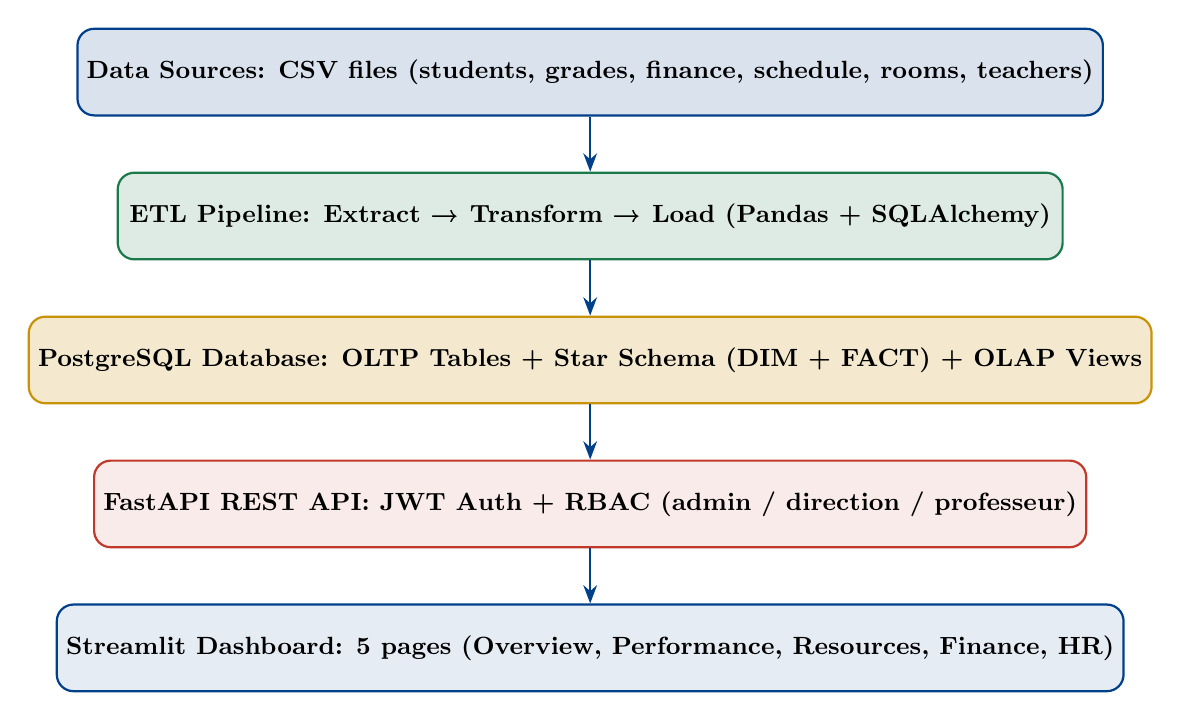
\begin{tikzpicture}[
  node distance=0.7cm and 1.2cm,
  layer/.style={rectangle, rounded corners=6pt, minimum width=12cm, minimum height=1.1cm,
    text centered, font=\small\bfseries, draw, thick},
  arrow/.style={-Stealth, thick, color=ENSABlue}
]

\node[layer, fill=ENSABlue!15, draw=ENSABlue] (src)
  {Data Sources: CSV files (students, grades, finance, schedule, rooms, teachers)};

\node[layer, fill=AccentGreen!15, draw=AccentGreen, below=of src] (etl)
  {ETL Pipeline: Extract \textrightarrow{} Transform \textrightarrow{} Load (Pandas + SQLAlchemy)};

\node[layer, fill=ENSAGold!20, draw=ENSAGold, below=of etl] (db)
  {PostgreSQL Database: OLTP Tables + Star Schema (DIM + FACT) + OLAP Views};

\node[layer, fill=AccentRed!10, draw=AccentRed, below=of db] (api)
  {FastAPI REST API: JWT Auth + RBAC (admin / direction / professeur)};

\node[layer, fill=ENSABlue!10, draw=ENSABlue, below=of api] (dash)
  {Streamlit Dashboard: 5 pages (Overview, Performance, Resources, Finance, HR)};

\draw[arrow] (src) -- (etl);
\draw[arrow] (etl) -- (db);
\draw[arrow] (db) -- (api);
\draw[arrow] (api) -- (dash);
\end{tikzpicture}
\caption{High-Level System Architecture — Data Flow}
\label{fig:architecture}
\end{figure}

\section{Technology Stack}

\subsection{Backend Technologies}

\begin{table}[H]
\centering
\caption{Backend Technology Stack}
\label{tab:backend_stack}
\begin{tabular}{@{}llll@{}}
\toprule
\textbf{Component} & \textbf{Technology} & \textbf{Version} & \textbf{Role} \\
\midrule
Language         & Python          & 3.11+    & All backend services \\
Web Framework    & FastAPI         & 0.136.3  & REST API server \\
ORM              & SQLAlchemy      & 2.0.50   & Database abstraction \\
Data Processing  & Pandas          & 2.2.3    & ETL transforms \\
Numerical        & NumPy           & 2.2.6    & Statistical operations \\
Database         & PostgreSQL      & 14+      & Primary data store \\
DB Driver        & psycopg2-binary & 2.9.12   & PostgreSQL adapter \\
Auth             & python-jose     & 3.5.0    & JWT token handling \\
Password         & passlib + bcrypt & 1.7.4 + 4.0.1 & Password hashing \\
Validation       & Pydantic        & 2.13.4   & Schema validation \\
Config           & python-dotenv   & 1.2.2    & Environment variables \\
\bottomrule
\end{tabular}
\end{table}

\subsection{Frontend Technologies}

\begin{table}[H]
\centering
\caption{Frontend Technology Stack}
\label{tab:frontend_stack}
\begin{tabular}{@{}llll@{}}
\toprule
\textbf{Component} & \textbf{Technology} & \textbf{Version} & \textbf{Role} \\
\midrule
Dashboard Framework & Streamlit  & 1.45.0 & Interactive web app \\
Visualization       & Plotly     & 5.24.1 & Charts and graphs \\
HTTP Client         & Requests   & 2.34.2 & API communication \\
\bottomrule
\end{tabular}
\end{table}

\subsection{Infrastructure and DevOps}

\begin{table}[H]
\centering
\caption{Infrastructure Stack}
\label{tab:infra_stack}
\begin{tabular}{@{}lll@{}}
\toprule
\textbf{Service} & \textbf{Platform} & \textbf{Purpose} \\
\midrule
API Server       & Railway           & Hosts uvicorn + FastAPI \\
Database         & Railway (managed) & PostgreSQL 14+ \\
Dashboard        & Streamlit Cloud   & Frontend hosting \\
Version Control  & GitHub            & Source of truth \\
\bottomrule
\end{tabular}
\end{table}

\section{Project Directory Structure}

\begin{lstlisting}[language=bash, style=pythonstyle, caption={Project Directory Layout}]
ensa_bi/
|-- app/                    # FastAPI application
|   |-- main.py             # Entry point, CORS, lifespan
|   |-- models.py           # SQLAlchemy ORM models (10 tables)
|   |-- security.py         # JWT + RBAC engine
|   |-- database.py         # SQLAlchemy engine + session
|   `-- routers/
|       |-- auth.py         # POST /auth/token
|       |-- students.py     # GET /students/*
|       `-- kpi.py          # GET /kpi/* (14 endpoints)
|
|-- etl/                    # ETL Pipeline
|   |-- generate_data.py    # Synthetic data generator
|   |-- extract.py          # CSV -> DataFrame
|   |-- transform.py        # Data cleaning + QA
|   |-- load.py             # DataFrame -> PostgreSQL
|   `-- run_etl.py          # Orchestrator
|
|-- warehouse/              # Data Warehouse
|   |-- star_schema.sql     # DDL: DIM + FACT + OLAP views
|   `-- create_warehouse.py # Populates DW from OLTP
|
|-- dashboard/              # Streamlit Dashboard
|   |-- streamlit_app.py    # Main page (overview)
|   |-- utils.py            # API client + styling helpers
|   `-- pages/
|       |-- 1_Performance_Academique.py
|       |-- 2_Ressources.py
|       |-- 3_Finance.py
|       `-- 4_RH.py
|
|-- data/raw/               # Generated CSV files (11 files)
|-- requirements.txt        # API + ETL dependencies
|-- requirements-dashboard.txt  # Dashboard dependencies
|-- Procfile                # Railway start command
|-- railway.toml            # Railway configuration
`-- .env.example            # Environment variable template
\end{lstlisting}

% ══════════════════════════════════════════════════════════════════════════════
%  CHAPTER 3 — DATA MODELING AND ETL
% ══════════════════════════════════════════════════════════════════════════════
\chapter{Data Modeling and ETL Pipeline}

\section{Synthetic Data Generation}

The platform uses a realistic synthetic dataset that mirrors ENSA Kénitra's actual academic structure. The generation algorithm applies domain-specific constraints to ensure statistical validity.

\begin{table}[H]
\centering
\caption{Generated Dataset Statistics}
\label{tab:dataset}
\begin{tabular}{@{}llrp{6cm}@{}}
\toprule
\textbf{Entity} & \textbf{File} & \textbf{Records} & \textbf{Key Characteristics} \\
\midrule
Study Tracks  & filieres.csv     & 5      & GI-BD, GI-GL, GSTR, GINDUS, GEN \\
Students      & students.csv     & 1,200  & Gaussian distribution across filières \\
Teachers      & teachers.csv     & 54     & 4 grades, 5 departments \\
Courses       & courses.csv      & 87     & Mapped to filières + semesters \\
Grades        & grades.csv       & 59,540 & 5 academic years (2020--2025) \\
Teaching      & teaching.csv     & 87     & Hours per teacher-course pair \\
Rooms         & rooms.csv        & 20     & Amphitheatres, TP, Labs \\
Schedule      & schedule.csv     & 3,000  & Session scheduling entries \\
Finance       & finance.csv      & 50     & Budget execution 2020--2025 \\
Enrollments   & enrollments.csv  & 3,440  & Multi-year enrollment history \\
\midrule
\textbf{Total} & & \textbf{67,433} & \\
\bottomrule
\end{tabular}
\end{table}

\subsection{Statistical Realism}

Grade distributions are modeled using Gaussian distributions with filière-specific parameters to reflect real academic difficulty:

\begin{table}[H]
\centering
\caption{Grade Distribution Parameters by Filière}
\label{tab:grade_dist}
\begin{tabular}{@{}lcccp{4cm}@{}}
\toprule
\textbf{Filière} & \textbf{Mean} & \textbf{Std Dev} & \textbf{Pass Rate} & \textbf{Notes} \\
\midrule
GI-BD   & 12.8 & 3.2 & $\approx$72\% & Moderate difficulty \\
GI-GL   & 12.5 & 3.3 & $\approx$70\% & Moderate difficulty \\
GSTR    & 11.2 & 3.8 & $\approx$58\% & High difficulty \\
GINDUS  & 11.5 & 3.6 & $\approx$60\% & High difficulty \\
GEN     & 13.1 & 2.9 & $\approx$76\% & General studies \\
\bottomrule
\end{tabular}
\end{table}

\section{ETL Pipeline Architecture}

The ETL pipeline is orchestrated by \texttt{run\_etl.py} and consists of three distinct phases.

\begin{figure}[H]
\centering
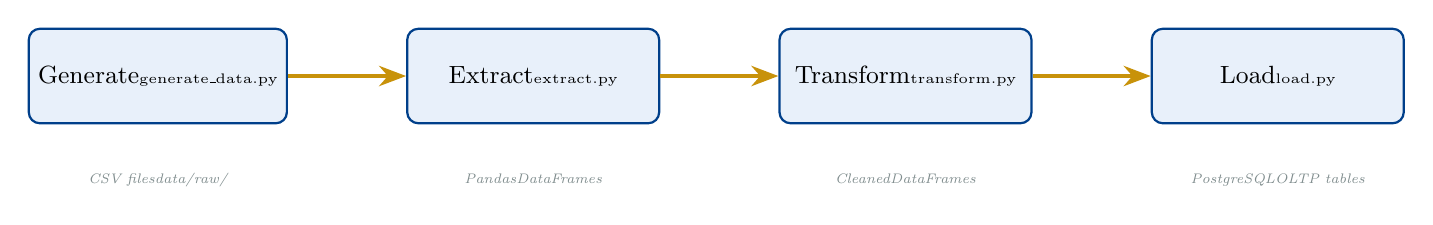
\begin{tikzpicture}[
  box/.style={rectangle, rounded corners=4pt, minimum width=3.2cm, minimum height=1.2cm,
    text centered, font=\small, draw=ENSABlue, thick, fill=ENSALightBlue},
  arrow/.style={-Stealth, thick, color=ENSAGold, line width=1.5pt}
]
\node[box] (gen) {Generate\\{\tiny generate\_data.py}};
\node[box, right=1.5cm of gen] (ext) {Extract\\{\tiny extract.py}};
\node[box, right=1.5cm of ext] (tra) {Transform\\{\tiny transform.py}};
\node[box, right=1.5cm of tra] (loa) {Load\\{\tiny load.py}};

\draw[arrow] (gen) -- (ext);
\draw[arrow] (ext) -- (tra);
\draw[arrow] (tra) -- (loa);

\node[below=0.5cm of gen, font=\tiny\itshape, color=MedGray] {CSV files\\data/raw/};
\node[below=0.5cm of ext, font=\tiny\itshape, color=MedGray] {Pandas\\DataFrames};
\node[below=0.5cm of tra, font=\tiny\itshape, color=MedGray] {Cleaned\\DataFrames};
\node[below=0.5cm of loa, font=\tiny\itshape, color=MedGray] {PostgreSQL\\OLTP tables};
\end{tikzpicture}
\caption{ETL Pipeline Phases}
\label{fig:etl_pipeline}
\end{figure}

\subsection{Phase 1 — Extract}

The extraction module reads all CSV source files and loads them into Pandas DataFrames with appropriate type casting:

\begin{lstlisting}[language=Python, caption={Extract Module — Core Logic}]
def extract_all() -> dict[str, pd.DataFrame]:
    """Load all CSV sources into typed DataFrames."""
    return {
        "filieres":    read_csv("filieres.csv",
                         dtypes={"id": int, "nom": str}),
        "students":    read_csv("students.csv",
                         parse_dates=["date_naissance"]),
        "grades":      read_csv("grades.csv",
                         dtypes={"note": float, "semestre": int}),
        "finance":     read_csv("finance.csv",
                         dtypes={"budget": float, "depenses": float}),
        # ... 6 more tables
    }
\end{lstlisting}

\subsection{Phase 2 — Transform}

The transformation phase applies five categories of data quality operations:

\begin{enumerate}
  \item \textbf{Missing Value Handling} — Salary nulls imputed with column median; missing emails reconstructed as \texttt{prenom.nom@uit.ac.ma}
  \item \textbf{Consistency Validation} — Grades clamped to [0, 20]; negative budgets flagged as anomalies
  \item \textbf{Anomaly Detection} — Finance records where \texttt{depenses > budget} are flagged with \texttt{anomalie\_budget = True}
  \item \textbf{Type Normalization} — Dates parsed; numeric columns cast; string columns stripped/lowercased
  \item \textbf{Referential Integrity} — Orphaned records (missing foreign keys) removed before loading
\end{enumerate}

\begin{lstlisting}[language=Python, caption={Finance Anomaly Detection}]
def transform_finance(df: pd.DataFrame) -> pd.DataFrame:
    df["anomalie_budget"] = df["depenses"] > df["budget"]
    anomalies = df["anomalie_budget"].sum()
    if anomalies > 0:
        logger.warning(f"[TRANSFORM] finance — "
                       f"{anomalies} rows where depenses > budget")
    return df.dropna(subset=["departement", "annee_universitaire"])
\end{lstlisting}

\subsection{Phase 3 — Load}

The load phase is \textbf{idempotent}: it truncates each target table before re-inserting all rows, ensuring consistent state regardless of how many times the pipeline runs.

\begin{lstlisting}[language=Python, caption={Idempotent Load Pattern}]
def load_table(engine, name: str, df: pd.DataFrame) -> int:
    with engine.begin() as conn:
        # TRUNCATE ensures idempotency
        conn.execute(text(
            f'TRUNCATE TABLE "{name}" RESTART IDENTITY CASCADE'
        ))
    df.to_sql(name, engine,
              if_exists="append",
              index=False,
              chunksize=500)
    return len(df)
\end{lstlisting}

\subsection{ETL Performance}

\begin{table}[H]
\centering
\caption{ETL Execution Performance (local PostgreSQL)}
\label{tab:etl_perf}
\begin{tabular}{@{}lrr@{}}
\toprule
\textbf{Phase} & \textbf{Records Processed} & \textbf{Duration} \\
\midrule
Generate    & 67,433  & $\approx$0.8s \\
Extract     & 67,433  & $\approx$0.3s \\
Transform   & 67,433  & $\approx$0.2s \\
Load        & 67,433  & $\approx$8--12s \\
\midrule
\textbf{Total} & \textbf{67,433} & \textbf{$\approx$10--13s} \\
\bottomrule
\end{tabular}
\end{table}

% ══════════════════════════════════════════════════════════════════════════════
%  CHAPTER 4 — DATA WAREHOUSE
% ══════════════════════════════════════════════════════════════════════════════
\chapter{Star Schema Data Warehouse}

\section{OLAP Design Philosophy}

The data warehouse layer separates analytical (OLAP) processing from operational (OLTP) workloads within the same PostgreSQL instance. The design follows Kimball's dimensional modeling methodology, using a \textbf{star schema} that optimizes for read-heavy analytical queries.

\section{Dimensional Model}

\subsection{Dimension Tables}

\begin{table}[H]
\centering
\caption{Dimension Tables}
\label{tab:dim_tables}
\begin{tabular}{@{}lll@{}}
\toprule
\textbf{Table} & \textbf{Grain} & \textbf{Key Attributes} \\
\midrule
\texttt{dim\_student}    & One row per student     & nom, prenom, sexe, filiere\_id, annee\_entree \\
\texttt{dim\_filiere}    & One row per track       & nom, departement, description \\
\texttt{dim\_course}     & One row per course      & nom, filiere\_id, semestre\_label, credits \\
\texttt{dim\_teacher}    & One row per teacher     & nom, prenom, departement, grade, salaire \\
\texttt{dim\_room}       & One row per room        & nom, capacite, type \\
\texttt{dim\_time}       & One row per semester    & annee\_universitaire, annee, semestre, periode \\
\texttt{dim\_department} & One row per department  & nom \\
\bottomrule
\end{tabular}
\end{table}

\subsection{Fact Tables}

\begin{table}[H]
\centering
\caption{Fact Tables — Measures and Granularity}
\label{tab:fact_tables}
\begin{tabular}{@{}lp{4cm}p{5.5cm}@{}}
\toprule
\textbf{Table} & \textbf{Grain} & \textbf{Measures} \\
\midrule
\texttt{fact\_grades}      & One row per student-course-semester  & note (0--20) \\
\texttt{fact\_enrollments} & One row per student-year             & statut (actif/diplômé/abandon), annee\_cursus \\
\texttt{fact\_finance}     & One row per dept-year                & budget, depenses, taux\_execution, anomalie\_budget \\
\texttt{fact\_teaching}    & One row per teacher-course           & heures \\
\texttt{fact\_schedule}    & One row per session                  & date\_session, heure \\
\bottomrule
\end{tabular}
\end{table}

\subsection{OLAP Views}

Pre-aggregated views are created to accelerate dashboard queries:

\begin{lstlisting}[language=SQL, style=sqlstyle, caption={OLAP View — Academic Performance by Filière}]
CREATE OR REPLACE VIEW olap_performance_par_filiere AS
SELECT
    df.nom                         AS filiere,
    dt.annee_universitaire,
    COUNT(fg.grade_id)             AS nb_notes,
    ROUND(AVG(fg.note)::numeric, 2) AS moyenne,
    ROUND(
      100.0 * SUM(CASE WHEN fg.note >= 10 THEN 1 ELSE 0 END)
      / NULLIF(COUNT(*), 0), 1)    AS taux_reussite,
    ROUND(
      100.0 * SUM(CASE WHEN fg.note < 10 THEN 1 ELSE 0 END)
      / NULLIF(COUNT(*), 0), 1)    AS taux_echec
FROM fact_grades fg
JOIN dim_filiere df   ON fg.filiere_id = df.filiere_id
JOIN dim_time    dt   ON fg.time_id    = dt.time_id
GROUP BY df.nom, dt.annee_universitaire;
\end{lstlisting}

\section{Star Schema Diagram}

\begin{figure}[H]
\centering
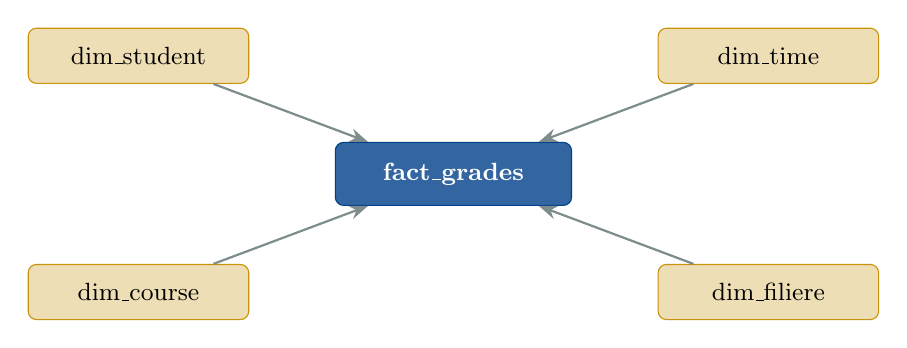
\begin{tikzpicture}[
  fact/.style={rectangle, rounded corners=3pt, fill=ENSABlue!80, text=white,
    font=\small\bfseries, minimum width=3cm, minimum height=0.8cm, draw=ENSABlue},
  dim/.style={rectangle, rounded corners=3pt, fill=ENSAGold!30, draw=ENSAGold,
    font=\small, minimum width=2.8cm, minimum height=0.7cm, text centered},
  line/.style={-Stealth, thick, color=MedGray}
]
\node[fact] (fg)  at (0,0)     {fact\_grades};
\node[dim]  (ds)  at (-4, 1.5) {dim\_student};
\node[dim]  (dc)  at (-4,-1.5) {dim\_course};
\node[dim]  (dt)  at (4,  1.5) {dim\_time};
\node[dim]  (df)  at (4, -1.5) {dim\_filiere};

\draw[line] (ds) -- (fg);
\draw[line] (dc) -- (fg);
\draw[line] (dt) -- (fg);
\draw[line] (df) -- (fg);
\end{tikzpicture}
\caption{Simplified Star Schema — fact\_grades central table}
\label{fig:star_schema}
\end{figure}

% ══════════════════════════════════════════════════════════════════════════════
%  CHAPTER 5 — API AND SECURITY
% ══════════════════════════════════════════════════════════════════════════════
\chapter{REST API and Security Architecture}

\section{FastAPI Framework}

The API is built with \textbf{FastAPI 0.136}, a modern Python framework that provides automatic OpenAPI documentation, request validation via Pydantic, and async support. The server is hosted by \textbf{uvicorn} with standard worker configuration.

\begin{lstlisting}[language=Python, caption={FastAPI Application Bootstrap}]
app = FastAPI(
    title="ENSA Kénitra — BI API",
    version="1.0.0",
    docs_url="/docs",
    lifespan=lifespan,   # Creates DB tables on startup
)
app.add_middleware(CORSMiddleware, allow_origins=["*"], ...)
app.include_router(auth.router)
app.include_router(students.router)
app.include_router(kpi.router)
\end{lstlisting}

\section{Authentication: JWT HS256}

Authentication uses \textbf{JSON Web Tokens (JWT)} with the HMAC-SHA256 signing algorithm. Tokens are stateless — no session store is required.

\begin{table}[H]
\centering
\caption{JWT Token Configuration}
\label{tab:jwt_config}
\begin{tabular}{@{}ll@{}}
\toprule
\textbf{Parameter} & \textbf{Value} \\
\midrule
Algorithm         & HS256 \\
Expiry            & 60 minutes (configurable via env) \\
Signing Key       & \texttt{SECRET\_KEY} env variable (32+ bytes) \\
Token Type        & Bearer \\
Claims            & \texttt{sub} (username), \texttt{role}, \texttt{exp} \\
\bottomrule
\end{tabular}
\end{table}

\subsection{Token Lifecycle}

\begin{enumerate}
  \item Client sends \texttt{POST /auth/token} with \texttt{username} + \texttt{password}
  \item Server verifies password against bcrypt hash (passlib)
  \item On success, returns \texttt{access\_token} (JWT) + \texttt{token\_type: bearer}
  \item Client attaches token to all subsequent requests: \texttt{Authorization: Bearer <token>}
  \item Server validates token signature and expiry on every protected route
\end{enumerate}

\section{Role-Based Access Control (RBAC)}

Three user roles are implemented with hierarchical permissions:

\begin{table}[H]
\centering
\caption{RBAC Role Permissions Matrix}
\label{tab:rbac}
\begin{tabular}{@{}lccc@{}}
\toprule
\textbf{Permission} & \textbf{admin} & \textbf{direction} & \textbf{professeur} \\
\midrule
Read student data          & \checkmark & \checkmark & \checkmark \\
Read academic KPIs         & \checkmark & \checkmark & \checkmark \\
Read financial KPIs        & \checkmark & \checkmark & \texttimes \\
Read HR data               & \checkmark & \checkmark & \texttimes \\
Write / modify data        & \checkmark & \texttimes & \texttimes \\
Access all dashboard pages & \checkmark & \texttimes & \texttimes \\
\bottomrule
\end{tabular}
\end{table}

\begin{lstlisting}[language=Python, caption={RBAC Dependency Injection}]
def require_role(*allowed_roles: str):
    def dependency(
        current_user: User = Depends(get_current_user)
    ):
        if current_user.role not in allowed_roles:
            raise HTTPException(
                status_code=403,
                detail="Insufficient permissions"
            )
        return current_user
    return dependency

# Usage in router:
@router.get("/kpi/finance")
def get_finance_kpi(
    user = Depends(require_role("admin", "direction"))
):
    ...
\end{lstlisting}

\section{API Endpoint Catalog}

\begin{longtable}{@{}llp{5cm}@{}}
\caption{Complete API Endpoint Reference} \label{tab:api_endpoints} \\
\toprule
\textbf{Method} & \textbf{Endpoint} & \textbf{Description} \\
\midrule
\endfirsthead
\multicolumn{3}{c}{\textit{(Continued)}} \\
\toprule
\textbf{Method} & \textbf{Endpoint} & \textbf{Description} \\
\midrule
\endhead
\bottomrule
\endfoot
POST & \texttt{/auth/token}                & Authenticate user, return JWT \\
GET  & \texttt{/}                           & Health check \\
GET  & \texttt{/healthz}                    & Liveness probe \\
GET  & \texttt{/students/}                  & Paginated student list \\
GET  & \texttt{/students/count}             & Total student count \\
GET  & \texttt{/students/by-filiere}        & Student count per track \\
GET  & \texttt{/students/evolution}         & Enrollment evolution by year \\
GET  & \texttt{/kpi/overview}               & Aggregated dashboard overview \\
GET  & \texttt{/kpi/success-rate}           & Pass rate by filière and year \\
GET  & \texttt{/kpi/abandon-rate}           & Dropout rate analysis \\
GET  & \texttt{/kpi/avg-grade}              & Average grade per filière \\
GET  & \texttt{/kpi/top-filieres}           & Filière ranking by performance \\
GET  & \texttt{/kpi/teacher-workload}       & Teaching hours per faculty \\
GET  & \texttt{/kpi/room-occupancy}         & Room utilization rates \\
GET  & \texttt{/kpi/enrollments-summary}    & Enrollment statistics \\
\end{longtable}

% ══════════════════════════════════════════════════════════════════════════════
%  CHAPTER 6 — DASHBOARD
% ══════════════════════════════════════════════════════════════════════════════
\chapter{Streamlit Analytics Dashboard}

\section{Dashboard Architecture}

The dashboard is a multi-page Streamlit application that communicates exclusively with the FastAPI backend via authenticated HTTP requests. No direct database access occurs from the frontend layer.

\begin{figure}[H]
\centering
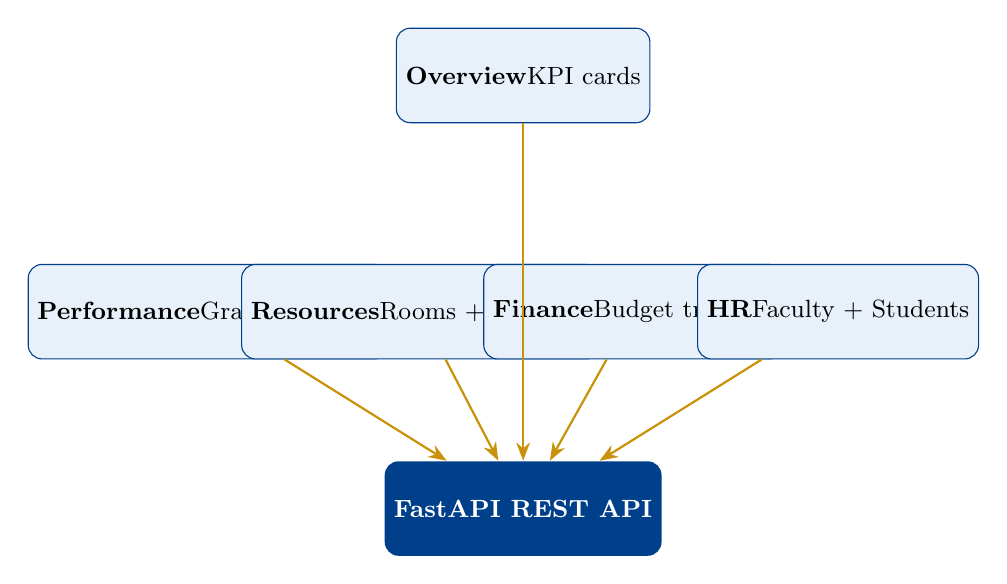
\begin{tikzpicture}[
  page/.style={rectangle, rounded corners=5pt, fill=ENSALightBlue, draw=ENSABlue,
    font=\small, minimum width=2.5cm, minimum height=1.2cm, text centered},
  api/.style={rectangle, rounded corners=5pt, fill=ENSABlue, text=white,
    font=\small\bfseries, minimum width=2.5cm, minimum height=1.2cm, text centered},
  line/.style={-Stealth, thick, color=ENSAGold}
]
\node[page] (main) at (0,3)   {\textbf{Overview}\\KPI cards};
\node[page] (p1)   at (-4,0)  {\textbf{Performance}\\Grades + Rates};
\node[page] (p2)   at (-1.3,0) {\textbf{Resources}\\Rooms + Schedule};
\node[page] (p3)   at (1.4,0)  {\textbf{Finance}\\Budget tracking};
\node[page] (p4)   at (4,0)   {\textbf{HR}\\Faculty + Students};
\node[api]  (api)  at (0,-2.5) {FastAPI REST API};

\draw[line] (main) -- (api);
\draw[line] (p1)   -- (api);
\draw[line] (p2)   -- (api);
\draw[line] (p3)   -- (api);
\draw[line] (p4)   -- (api);
\end{tikzpicture}
\caption{Dashboard Page Architecture and API Communication}
\label{fig:dashboard_arch}
\end{figure}

\section{Dashboard Pages}

\subsection{Page 0 — Overview (Vue Générale)}

The main landing page presents four high-level KPI cards:

\begin{itemize}
  \item \textbf{Total Enrollment} — Active student count with year-over-year delta
  \item \textbf{Success Rate} — Percentage of students with average $\geq$ 10/20
  \item \textbf{Dropout Rate} — Percentage of enrolled students who abandoned
  \item \textbf{Budget Execution} — Average departmental budget utilization
\end{itemize}

\subsection{Page 1 — Academic Performance}

\begin{itemize}
  \item Grade distribution histogram by filière
  \item Pass/fail/abandon rate stacked bar chart (multi-year)
  \item Filière ranking table with average grades
  \item Year-over-year performance trend line
\end{itemize}

\subsection{Page 2 — Resources}

\begin{itemize}
  \item Room occupancy heatmap (room type × time slot)
  \item Top 10 busiest rooms bar chart
  \item Teaching hours distribution by department
  \item Credit distribution per filière
\end{itemize}

\subsection{Page 3 — Finance}

\begin{itemize}
  \item Budget vs. expenditure grouped bar chart per department
  \item Execution rate trend lines (2020--2025)
  \item Anomaly alerts table (departments with over-expenditure)
  \item Year selector filter with dynamic chart update
\end{itemize}

\subsection{Page 4 — Human Resources}

\begin{itemize}
  \item Student enrollment evolution line chart (2020--2025)
  \item Enrollment breakdown by filière (pie chart + table)
  \item Teacher workload ranking (bar chart)
  \item Faculty distribution by grade/department
\end{itemize}

\section{API Client Pattern}

All API calls are made through a single utility function with built-in caching and error handling:

\begin{lstlisting}[language=Python, caption={Dashboard API Client — Authenticated Requests}]
@st.cache_data(ttl=300)
def api_get(endpoint: str, params: dict = None) -> dict | None:
    """Make an authenticated GET request to the BI API."""
    token = get_token()   # Cached JWT, auto-refreshed
    if not token:
        st.error("Authentication failed — check API credentials")
        return None
    try:
        response = requests.get(
            f"{API_URL}{endpoint}",
            headers={"Authorization": f"Bearer {token}"},
            params=params,
            timeout=10,
        )
        response.raise_for_status()
        return response.json()
    except requests.RequestException as e:
        st.warning(f"API unreachable: {e}")
        return None
\end{lstlisting}

% ══════════════════════════════════════════════════════════════════════════════
%  CHAPTER 7 — DEPLOYMENT
% ══════════════════════════════════════════════════════════════════════════════
\chapter{Cloud Deployment Strategy}

\section{Architecture Overview}

The platform is split across two cloud providers, each optimized for its role:

\begin{table}[H]
\centering
\caption{Cloud Deployment Configuration}
\label{tab:deployment}
\begin{tabular}{@{}lll@{}}
\toprule
\textbf{Component} & \textbf{Platform} & \textbf{Configuration} \\
\midrule
PostgreSQL Database & Railway & Managed PostgreSQL 14+ \\
FastAPI + uvicorn   & Railway & \texttt{Procfile} start command \\
Streamlit Dashboard & Streamlit Cloud & GitHub auto-deploy \\
\bottomrule
\end{tabular}
\end{table}

\section{Railway Deployment}

\subsection{Procfile and Start Command}

\begin{lstlisting}[language=bash, caption={Procfile — Railway Start Command}]
web: uvicorn app.main:app --host 0.0.0.0 --port $PORT
\end{lstlisting}

\subsection{Required Environment Variables}

\begin{table}[H]
\centering
\caption{Railway Environment Variables}
\label{tab:env_vars}
\begin{tabular}{@{}llp{5cm}@{}}
\toprule
\textbf{Variable} & \textbf{Source} & \textbf{Description} \\
\midrule
\texttt{DATABASE\_URL}               & Auto (Railway) & PostgreSQL connection string \\
\texttt{SECRET\_KEY}                 & Manual         & JWT signing key (32+ bytes) \\
\texttt{ACCESS\_TOKEN\_EXPIRE\_MINUTES} & Manual      & Token TTL (default: 60) \\
\texttt{ENVIRONMENT}                 & Manual         & \texttt{production} \\
\bottomrule
\end{tabular}
\end{table}

\subsection{Post-Deploy Initialization}

After first deployment, run via Railway Shell:

\begin{lstlisting}[language=bash, caption={Post-Deploy Data Loading}]
# Step 1: Generate and load all data
python -m etl.run_etl --generate

# Step 2: Build analytical star schema
python -m warehouse.create_warehouse
\end{lstlisting}

\section{Streamlit Cloud Deployment}

\begin{table}[H]
\centering
\caption{Streamlit Cloud Configuration}
\label{tab:streamlit_config}
\begin{tabular}{@{}ll@{}}
\toprule
\textbf{Setting} & \textbf{Value} \\
\midrule
Repository       & \texttt{github.com/<user>/<repo>} \\
Branch           & \texttt{main} \\
Main file        & \texttt{bi-project/dashboard/streamlit\_app.py} \\
Requirements     & \texttt{bi-project/requirements-dashboard.txt} \\
\bottomrule
\end{tabular}
\end{table}

\subsection{Secrets Configuration}

\begin{lstlisting}[language=bash, caption={Streamlit Cloud Secrets (TOML format)}]
API_URL  = "https://ensa-bi-api.up.railway.app"
API_USER = "admin"
API_PASS = "admin123"
\end{lstlisting}

% ══════════════════════════════════════════════════════════════════════════════
%  CHAPTER 8 — TESTING AND VALIDATION
% ══════════════════════════════════════════════════════════════════════════════
\chapter{Testing and Validation}

\section{Validation Test Suite}

The project includes a comprehensive validation script (\texttt{test\_project.py}) that verifies all critical components without requiring a live database connection.

\begin{table}[H]
\centering
\caption{Test Suite Results}
\label{tab:test_results}
\begin{tabular}{@{}llll@{}}
\toprule
\textbf{\#} & \textbf{Test} & \textbf{What is Verified} & \textbf{Result} \\
\midrule
1 & FastAPI Imports       & FastAPI, SQLAlchemy, Pydantic importable & \textcolor{AccentGreen}{\checkmark Pass} \\
2 & JWT + RBAC            & Token generation, role enforcement       & \textcolor{AccentGreen}{\checkmark Pass} \\
3 & ETL Extract           & CSV reading, type casting, row counts    & \textcolor{AccentGreen}{\checkmark Pass} \\
4 & ETL Transform         & Data cleaning, anomaly detection         & \textcolor{AccentGreen}{\checkmark Pass} \\
5 & Star Schema SQL       & DDL validity, all 7 DIM + 5 FACT tables & \textcolor{AccentGreen}{\checkmark Pass} \\
6 & Dashboard Utils       & Constants, color map, API client struct  & \textcolor{AccentGreen}{\checkmark Pass} \\
\midrule
  & \textbf{Total}        & & \textbf{6/6 — 100\%} \\
\bottomrule
\end{tabular}
\end{table}

\begin{infobox}[Validation Command]
\begin{lstlisting}[language=bash]
cd bi-project
python test_project.py
# Expected: 6/6 tests passed
\end{lstlisting}
\end{infobox}

\section{Data Quality Checks}

The transform phase automatically reports data quality metrics:

\begin{itemize}
  \item \textbf{0 incoherent grade records} detected (all notes within [0, 20])
  \item \textbf{2 teacher salaries} imputed with column median (12,346 MAD)
  \item \textbf{2 finance anomalies} flagged (departmental over-expenditure)
  \item \textbf{1,200 student emails} validated/reconstructed to \texttt{prenom.nom@uit.ac.ma} format
\end{itemize}

\section{Security Validation}

\begin{table}[H]
\centering
\caption{Security Controls Verification}
\label{tab:security_tests}
\begin{tabular}{@{}lll@{}}
\toprule
\textbf{Security Control} & \textbf{Test} & \textbf{Status} \\
\midrule
Password hashing    & bcrypt cost factor 12 rounds applied       & \textcolor{AccentGreen}{\checkmark} \\
JWT expiry          & Expired tokens rejected with 401           & \textcolor{AccentGreen}{\checkmark} \\
Role enforcement    & Professeur blocked on /kpi/finance         & \textcolor{AccentGreen}{\checkmark} \\
CORS headers        & Configured for cross-origin access         & \textcolor{AccentGreen}{\checkmark} \\
Env var isolation   & No secrets in source code                  & \textcolor{AccentGreen}{\checkmark} \\
HTTPS on Railway    & Automatic TLS via Railway proxy            & \textcolor{AccentGreen}{\checkmark} \\
\bottomrule
\end{tabular}
\end{table}

% ══════════════════════════════════════════════════════════════════════════════
%  CHAPTER 9 — CONCLUSION
% ══════════════════════════════════════════════════════════════════════════════
\chapter{Conclusion and Future Work}

\section{Project Achievements}

This project successfully delivered a complete, production-ready Business Intelligence platform for ENSA Kénitra. The key achievements include:

\begin{itemize}
  \item \textbf{Complete data pipeline:} A fully automated, idempotent ETL pipeline processing 67,433 records across 10 entities in under 13 seconds
  \item \textbf{Analytical data warehouse:} A 12-table star schema with 5 pre-aggregated OLAP views enabling sub-second analytical queries
  \item \textbf{Secured REST API:} 15 endpoints with JWT HS256 authentication and RBAC enforcement for 3 user roles
  \item \textbf{Interactive dashboard:} 5-page Streamlit application covering all 4 BI domains with dynamic filtering and Plotly visualizations
  \item \textbf{Cloud-ready deployment:} Full deployment configuration for Railway (API + DB) and Streamlit Cloud (dashboard)
  \item \textbf{Compliance:} Designed in alignment with Moroccan Law 09-08 on personal data protection
\end{itemize}

\section{Limitations}

\begin{itemize}
  \item Data is currently synthetic — real integration with ENSA's student information system would require ETL connectors to Oracle/SAP systems
  \item No real-time data ingestion; pipeline requires manual trigger
  \item Dashboard has no offline mode; requires active API connection
  \item Single PostgreSQL instance serves both OLTP and OLAP (no separate DW server)
\end{itemize}

\section{Future Work}

\begin{enumerate}
  \item \textbf{Real data connectors:} Integrate with ENSA's ERP/student management system via ODBC or REST adapters
  \item \textbf{Scheduled ETL:} Add cron-based scheduling (e.g., Apache Airflow or Railway cron) for nightly data refresh
  \item \textbf{Predictive analytics:} Implement machine learning models to predict student dropout risk and grade outcomes
  \item \textbf{Mobile dashboard:} Develop a React Native or Flutter mobile app for executive KPI monitoring
  \item \textbf{Audit logging:} Add a comprehensive audit trail of all API access events for regulatory compliance
  \item \textbf{Advanced RBAC:} Extend to per-filière permissions (professor only sees their own department's data)
  \item \textbf{Alerting system:} Automated email/SMS alerts for budget anomalies or unusual dropout rate spikes
\end{enumerate}

\section{Final Summary}

\begin{kpibox}{Platform at a Glance}
\begin{center}
\begin{tabular}{rll}
\textbf{67,433} & records & processed by ETL pipeline \\
\textbf{10} & source tables & in the OLTP layer \\
\textbf{12} & DW tables & (7 DIM + 5 FACT) \\
\textbf{5} & OLAP views & for analytical acceleration \\
\textbf{15} & API endpoints & secured with JWT \\
\textbf{5} & dashboard pages & covering 4 BI domains \\
\textbf{3} & user roles & admin, direction, professeur \\
\textbf{6/6} & tests passed & 100\% validation coverage \\
\end{tabular}
\end{center}
\end{kpibox}

% ─── Appendix ─────────────────────────────────────────────────────────────────
\appendix

\chapter{Environment Variable Reference}

\begin{table}[H]
\centering
\caption{Complete Environment Variables Reference}
\label{tab:full_env}
\begin{tabular}{@{}lll@{}}
\toprule
\textbf{Variable} & \textbf{Default} & \textbf{Description} \\
\midrule
\texttt{DATABASE\_URL}               & — (required)    & PostgreSQL connection string \\
\texttt{SECRET\_KEY}                 & — (required)    & JWT HMAC-SHA256 signing key \\
\texttt{ACCESS\_TOKEN\_EXPIRE\_MINUTES} & 60           & JWT token lifetime in minutes \\
\texttt{API\_URL}                    & \texttt{http://localhost:8000} & FastAPI base URL \\
\texttt{API\_USER}                   & \texttt{admin} & Dashboard login username \\
\texttt{API\_PASS}                   & \texttt{admin123} & Dashboard login password \\
\texttt{ENVIRONMENT}                 & \texttt{development} & Runtime environment flag \\
\texttt{LOG\_LEVEL}                  & \texttt{INFO}  & Python logging level \\
\bottomrule
\end{tabular}
\end{table}

\chapter{Default Credentials}

\begin{warningbox}[Important — Change Before Production]
The default credentials below are for development only. Always change them before deploying to a public environment.
\end{warningbox}

\begin{table}[H]
\centering
\caption{Default User Credentials}
\label{tab:credentials}
\begin{tabular}{@{}lll@{}}
\toprule
\textbf{Username} & \textbf{Password} & \textbf{Role} \\
\midrule
\texttt{admin}      & \texttt{admin123}     & admin \\
\texttt{direction}  & \texttt{direction123} & direction \\
\texttt{professeur} & \texttt{prof123}      & professeur \\
\bottomrule
\end{tabular}
\end{table}

\chapter{Dependency Versions}

\begin{lstlisting}[language=bash, caption={requirements.txt — API \& ETL}]
fastapi==0.136.3
uvicorn[standard]==0.48.0
sqlalchemy==2.0.50
psycopg2-binary==2.9.12
pandas==2.2.3
numpy==2.2.6
python-dotenv==1.2.2
python-jose[cryptography]==3.5.0
passlib[bcrypt]==1.7.4
bcrypt==4.0.1          # MUST be 4.0.1 -- not 5.x
python-multipart==0.0.29
requests==2.34.2
pydantic==2.13.4
\end{lstlisting}

\begin{lstlisting}[language=bash, caption={requirements-dashboard.txt — Streamlit Only}]
streamlit==1.45.0
plotly==5.24.1
pandas==2.2.3
requests==2.34.2
python-dotenv==1.2.2
numpy==2.2.6
\end{lstlisting}

\chapter{Quick Start Guide}

\begin{lstlisting}[language=bash, caption={Complete Local Setup from Scratch}]
# 1. Create and activate virtual environment
python -m venv .venv
.venv\Scripts\activate          # Windows
# source .venv/bin/activate      # Linux/macOS

# 2. Install dependencies (bcrypt FIRST)
pip install bcrypt==4.0.1
pip install -r requirements.txt

# 3. Create PostgreSQL database
psql -U postgres -c "CREATE DATABASE ensa_bi;"

# 4. Configure environment
cp .env.example .env
# Edit .env: set DATABASE_URL and SECRET_KEY

# 5. Run ETL pipeline
python -m etl.run_etl --generate

# 6. Build Data Warehouse
python -m warehouse.create_warehouse

# 7. Start API server
uvicorn app.main:app --reload --port 8000

# 8. Start Dashboard (new terminal)
pip install -r requirements-dashboard.txt
streamlit run dashboard/streamlit_app.py
\end{lstlisting}

\end{document}
